\begin{figure}[H]
    \centering
    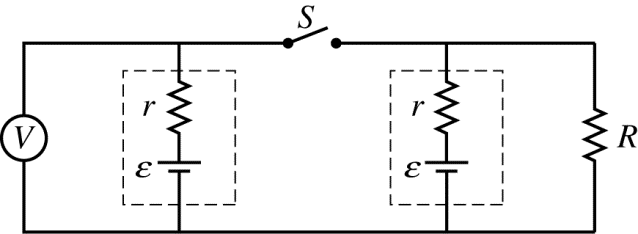
\includegraphics[scale=0.3]{images/img-008-013.png}
\end{figure}

% Multiple Choice Question 16
\begin{questions}\setcounter{question}{15}\question
A resistor of resistance $R$ is connected in a circuit to two identical batteries. The circuit also contains switch $S$ and ideal voltmeter $V$, as shown in the figure above. The batteries both have an emf $\varepsilon$ and internal resistance $r$. The reading of the voltmeter is noted with the switch in the open position. Which of the following best represents how the voltmeter reading after the switch is closed compares to the reading before the switch is closed?

\begin{choices}
\choice The reading of the voltmeter is the same.
\choice The reading of the voltmeter is higher.
\choice The reading of the voltmeter is lower.
\choice Cannot be determined without knowing the internal resistance of the batteries.
\choice Cannot be determined without knowing the emf of the batteries.
\end{choices}\end{questions}

